\chapter{Entrepreneurs: An Interesting Perspective on Building Wealth}

This short interview is organized around a single quantitative intuition. We begin with a practical question asked by an engineer, we are given an answer before we are given its proof, and then the proof is supplied by a few large numbers: the present scale of the world economy, its present dependence on fossil fuels, its projected size in 2050, and the added condition of net zero. The mathematics is light, but the structure is exact. Wealth, in this picture, forms where an immense system must both grow and change its basis.

\section{Opening Setup}

The conversation does not begin with a sermon about money. It begins with a career-allocation problem. The interviewer asks what industry one should pursue, then identifies himself as an engineer, and only then sharpens the issue into the wealth question. That order matters. We are not being asked what slogan to admire, nor even what asset to buy. We are being asked where a technically minded builder should go.

This framing gives the whole clip its discipline. The reply is not meant to be a sociological comment about the economy in general. It is meant to function as directional advice for someone deciding where to spend technical effort.

\section{The Wealth Question}

The speaker's next move is the most important rhetorical move in the interview: he answers first and justifies afterward. The thesis is stated before the machinery that supports it.

\subsection{Question \& Answer}

The question is direct: how can someone become wealthy in 2022?

The answer is just as direct: the next 1{,}000 unicorns will be in green tech.

We should not hear this as detached enthusiasm. In the structure of the clip, it is the conclusion placed in front of us before the premises are unfolded. The next lines are therefore not ornamental. They are the compact proof of why green tech is said to be ``the place to go.''

\section{The Present Baseline}

To justify the thesis, the speaker first fixes the present scale of the system. We may introduce a small amount of notation, explicitly as editorial shorthand for the spoken claims.

\begin{definition}
For \(t \in \{2022,2050\}\), let \(W_t\) denote the scale of the world economy, let \(f_{\mathrm{fossil},t}\) denote the rough fossil-fuel dependence of the system, and let \(E_{\mathrm{net},t}\) denote the net-emissions condition. These are not quoted lecture symbols; they are a compact way to keep the logic of the interview visible on the page.
\end{definition}

The first baseline number is the size of the world economy:
\begin{equation}
W_{2022} \approx \$90\text{ trillion}.
\end{equation}
The second is the stated dependence on fossil fuels:
\begin{equation}
f_{\mathrm{fossil},2022} \approx 0.8.
\end{equation}

These two statements do the real work of the setup. The first says that we are dealing with a civilization-scale economic machine, not a niche market. The second says that this machine still runs largely on a fossil base. The transition, then, is not something happening at the edge of the economy. It acts on the bulk of the system itself.

\begin{remark}
The \(80\%\) figure should be read cautiously. In the interview it serves as a rough indicator of fossil dependence, not as a carefully defined statistic with an explicit denominator. We preserve it for scale, not for false precision.
\end{remark}

\section{The 2050 Shift}

Once the present has been fixed, the speaker turns the argument forward in time. The future is not described as a cleaner version of the present. It is described as both larger and more constrained.

The time horizon is stated explicitly:
\begin{equation}
2050 - 2022 = 28.
\end{equation}
Over that horizon the world economy is said to double:
\begin{align}
W_{2050} &\approx 2W_{2022},\\
W_{2050} &\approx \$180\text{ trillion}.
\end{align}
At the same time, the future system is required to be net zero, which we may encode schematically as
\begin{equation}
E_{\mathrm{net},2050} \approx 0.
\end{equation}

Here the clip reaches its hinge. A larger economy alone would give us an expansion problem. Net zero alone would give us a conversion problem. The interview combines the two. The world must build a bigger productive order while displacing the dominant energy basis of the current one. That is the source of the commercial opportunity.

\begin{figure}
\centering
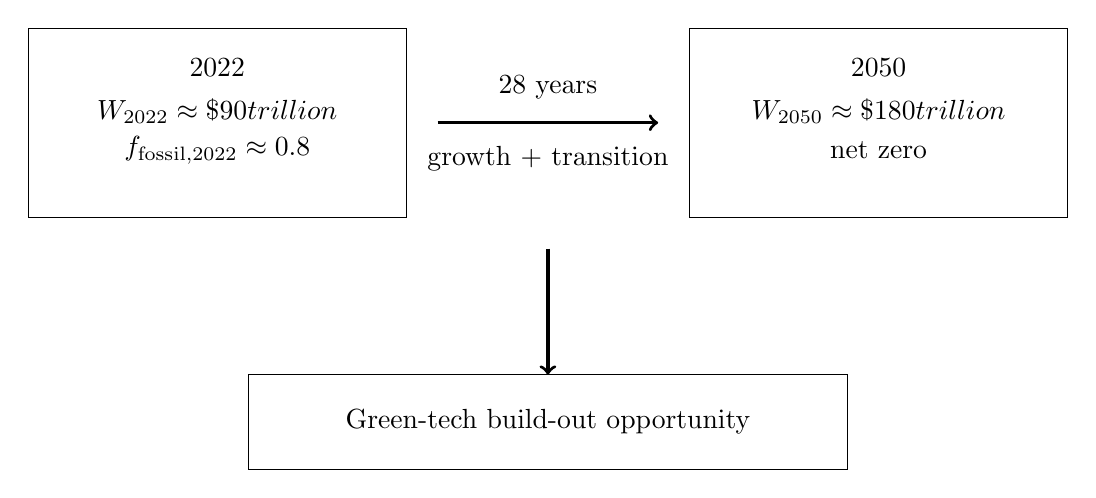
\begin{tikzpicture}[x=1cm,y=1cm]
\draw (0,0) rectangle (4.8,2.4);
\node at (2.4,1.9) {2022};
\node at (2.4,1.35) {$W_{2022}\approx \$90\text{ trillion}$};
\node at (2.4,0.85) {$f_{\mathrm{fossil},2022}\approx 0.8$};

\draw[->, very thick] (5.2,1.2) -- (8.0,1.2);
\node at (6.6,1.65) {$28$ years};
\node at (6.6,0.75) {growth + transition};

\draw (8.4,0) rectangle (13.2,2.4);
\node at (10.8,1.9) {2050};
\node at (10.8,1.35) {$W_{2050}\approx \$180\text{ trillion}$};
\node at (10.8,0.85) {net zero};

\draw[->, very thick] (6.6,-0.4) -- (6.6,-2.0);
\draw (2.8,-3.2) rectangle (10.4,-2.0);
\node at (6.6,-2.6) {Green-tech build-out opportunity};
\end{tikzpicture}
\end{figure}

We should read this figure as a schematic of the argument. Present scale, future scale, and the net-zero condition are not three separate observations. Together they define the shape of the opportunity.

\section{Transition Arithmetic}

At this point we can let the numbers speak to one another. The interview does not present a formal model, so what follows should be understood as a cautious worked estimate rather than an exact calculation.

\paragraph{Step 1: a rough present fossil-dependent scale.}

If we take the spoken \(80\%\) as a rough multiplier on present scale, then an order-of-magnitude estimate for the fossil-dependent portion of the current system is
\begin{align}
W_{\mathrm{fossil\text{-}dependent},2022}
&\approx f_{\mathrm{fossil},2022}W_{2022}\\
&\approx 0.8 \times \$90\text{ trillion}\\
&\approx \$72\text{ trillion}.
\end{align}

\paragraph{Step 2: a rough future increment in total scale.}

The same spoken numbers also imply a large growth increment:
\begin{align}
\Delta W
&\approx W_{2050} - W_{2022}\\
&\approx \$180\text{ trillion} - \$90\text{ trillion}\\
&\approx \$90\text{ trillion}.
\end{align}

\paragraph{Step 3: combine growth with conversion.}

The point is not that \(\$72\) trillion and \(\$90\) trillion can be added as if they were neat and non-overlapping accounting bins. The point is structural. We are asked to imagine, at once,
\begin{enumerate}
\item a very large existing productive base still tied to fossil energy, and
\item a very large further increment of output that must arrive under a net-zero condition.
\end{enumerate}

So the speaker's mechanism may be summarized schematically as
\begin{equation}
\bigl(W_{2050} \approx 2W_{2022}\bigr)
\land
\bigl(f_{\mathrm{fossil},2022} \approx 0.8\bigr)
\land
\bigl(E_{\mathrm{net},2050} \approx 0\bigr)
\Rightarrow
\text{large green-tech build-out opportunity}.
\end{equation}

This is not a theorem. It is the disciplined mathematical skeleton of the interview. Once we have a system this large that must both expand and decarbonize, the transition ceases to be a marginal adjustment. It becomes a vast design-and-deployment problem.

\section{Why This Points to Green Tech}

Now the opening answer becomes intelligible. The phrase ``the next 1{,}000 unicorns'' is not used here as the output of a valuation model. It is used to name a zone of concentrated firm formation. If an engineer asks where new, very large companies are most likely to arise, the speaker points toward the sector that must absorb both growth and conversion.

That is why the clip begins with engineering. The commercial conclusion is not merely that money will flow toward decarbonization in some abstract sense. It is that technical work will be required at every layer of the transition: generation, storage, transmission, industrial process, materials, software, finance, and deployment. The interview does not enumerate these layers, but the logic of the argument points toward them. Wealth will tend to form where technical difficulty and economic necessity are forced together.

The final recap in the transcript now lands with full force. The next 1{,}000 unicorns will be in green tech because a larger world economy must be made compatible with net zero. On this view, green tech is not one opportunity among many; it is where the scale of the problem makes large outcomes plausible.

\section{Summary}

The lecture unfolds in a clear order. A practical question is asked by an engineer. A sharp answer is given: green tech. That answer is then justified by four linked quantities or conditions: a \(\$90\) trillion present world economy, rough \(80\%\) fossil dependence, a doubling to \(\$180\) trillion by 2050, and a net-zero endpoint. From these, the speaker infers a very large build-out problem.

That is the chapter's mathematical spine. It is not a detailed climate model and not a formal theory of startup formation. It is a scale argument. When a system this large must both grow and transform, the search for wealth moves toward the industries that make the transformation possible. Green tech is presented as the most consequential instance of that rule, and therefore, in the speaker's closing phrase, as the place to go.